% Propósito: separar el efecto de un gradiente de viento del viento uniforme.
% Origen: c_ef(z)=c+u(z) cos(psi); los rayos se curvan hacia menor c_ef.
% Esquema cualitativo, sin datos meteorológicos.
% Accesibilidad: con sonido de izquierda a derecha, el viento a favor aumenta
% con la altura y curva los rayos hacia el suelo; en contra los curva hacia arriba.
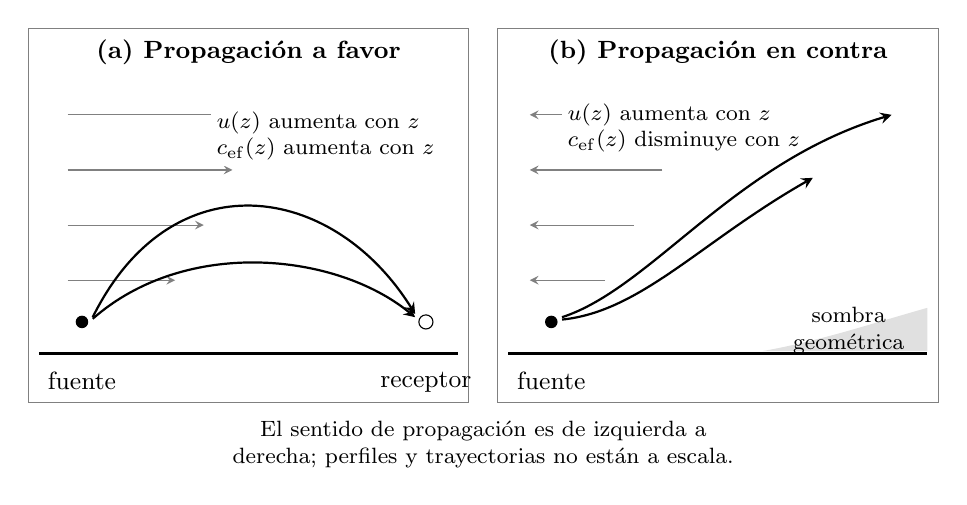
\begin{tikzpicture}[
    x=0.91cm,
    y=1cm,
    >=stealth,
    font=\small,
    rayo/.style={thick,->},
    viento/.style={gray,->},
    guia/.style={gray,dashed}
]
    % A favor
    \draw[gray] (0,0) rectangle (6.15,4.75);
    \node[font=\small\bfseries] at (3.075,4.45) {(a) Propagación a favor};
    \draw[thick] (0.15,0.62) -- (6.0,0.62);
    \node[fill=black,circle,inner sep=1.6pt] (sf) at (0.75,1.02) {};
    \node[anchor=north] at (0.75,0.50) {fuente};
    \node[draw,circle,inner sep=1.8pt] (rf) at (5.55,1.02) {};
    \node[anchor=north] at (5.55,0.50) {receptor};
    \foreach \y/\xend in {1.55/2.05,2.25/2.45,2.95/2.85,3.65/3.25}{
        \draw[viento] (0.55,\y) -- (\xend,\y);
    }
    \node[align=left,font=\footnotesize,fill=white,inner sep=2pt]
        at (4.15,3.38)
        {\(u(z)\) aumenta con \(z\)\\
         \(c_\mathrm{ef}(z)\) aumenta con \(z\)};
    \draw[rayo] (0.90,1.08)
        .. controls (2.00,3.10) and (4.25,2.80) .. (5.40,1.12);
    \draw[rayo] (0.90,1.06)
        .. controls (2.20,2.10) and (4.30,1.90) .. (5.40,1.08);

    % En contra
    \draw[gray] (6.55,0) rectangle (12.70,4.75);
    \node[font=\small\bfseries] at (9.625,4.45) {(b) Propagación en contra};
    \draw[thick] (6.70,0.62) -- (12.55,0.62);
    \node[fill=black,circle,inner sep=1.6pt] (sc) at (7.30,1.02) {};
    \node[anchor=north] at (7.30,0.50) {fuente};
    \foreach \y/\xend in {1.55/8.05,2.25/8.45,2.95/8.85,3.65/9.25}{
        \draw[viento] (\xend,\y) -- (7.00,\y);
    }
    \node[align=left,font=\footnotesize,fill=white,inner sep=2pt]
        at (9.15,3.48)
        {\(u(z)\) aumenta con \(z\)\\
         \(c_\mathrm{ef}(z)\) disminuye con \(z\)};
    \draw[rayo] (7.45,1.08)
        .. controls (8.70,1.45) and (9.85,3.05) .. (12.05,3.65);
    \draw[rayo] (7.45,1.05)
        .. controls (8.55,1.15) and (9.40,2.05) .. (10.95,2.85);
    \path[fill=black!12] (10.25,0.65) -- (12.55,0.65) -- (12.55,1.20)
        .. controls (11.70,0.98) and (11.05,0.78) .. cycle;
    \node[align=center,font=\footnotesize] at (11.45,0.91)
        {sombra\\geométrica};

    \node[font=\footnotesize,anchor=north,text width=11cm,align=center]
        at (6.35,-0.12)
        {El sentido de propagación es de izquierda a derecha; perfiles y trayectorias no están a escala.};
\end{tikzpicture}
